\documentclass[11pt,a4paper,twoside]{book}

% Input encoding and basic packages
\usepackage[utf8]{inputenc}
\usepackage[english]{babel} % Replace "english" with your document language
\usepackage{graphicx}
\usepackage{amsmath, amssymb}
\usepackage{tcolorbox}
\usepackage{xcolor}
\usepackage{geometry}
\usepackage{wrapfig}
\usepackage{titlesec}
\usepackage{fancyhdr}
\usepackage{caption}
\usepackage{float}
\usepackage{hyperref}
\usepackage{subcaption}
\usepackage{fontspec}
\usepackage{nomencl} 
\usepackage{multicol}
\usepackage{etoolbox}
\usepackage{microtype}


% Fonts
\setmainfont{Poppins} % Main font for body text
\newfontfamily\titlesfont{Anonymous Pro} % Font for titles

% Relax Latex rules for text layout
\raggedbottom
\sloppy
\raggedright

% \emergencystretch=1em % Allows LaTeX to stretch text slightly to avoid gaps
% \tolerance=2000 % Sets the general tolerance level
% \hbadness=1000 % Suppresses warnings for "bad" spacing

% Define custom colors
\definecolor{cherenkovblue}{RGB}{55, 139, 230}
\definecolor{white}{RGB}{255, 255, 255}

% Adjust default font sizes
\renewcommand{\normalsize}{\fontsize{9}{11}\selectfont} % Smaller body text: 9pt font with 11pt line spacing
\renewcommand{\small}{\fontsize{8}{10}\selectfont}
\renewcommand{\footnotesize}{\fontsize{7}{9}\selectfont}

% Title styling
\titleformat{\title}{\color{cherenkovblue}\titlesfont\huge\bfseries}{\thetitle}{1em}{}
\titleformat{\part}{\color{cherenkovblue}\titlesfont\huge\bfseries}{\thepart}{1em}{}
\titleformat{\chapter}{\color{cherenkovblue}\titlesfont\Huge\bfseries}{\thechapter}{0.5em}{}[\vspace{-2ex}]
\titleformat{\section}{\color{cherenkovblue}\titlesfont\Large\bfseries}{\thesection}{1em}{}
\titleformat{\subsection}{\color{cherenkovblue}\titlesfont\large\bfseries}{\thesubsection}{1em}{}
\titleformat{\paragraph}{\bfseries}{\theparagraph}{1em}{}

% Remove indentation
\setlength{\parindent}{0pt}
\setlength{\parskip}{6pt} % Add spacing between paragraphs

% Customize itemize bullets
\renewcommand\labelitemi{--} % Use dashes instead of bullets

% Define box styles
\tcbset{
    boxstyle/.style={
        colframe=cherenkovblue,
        colback=white,
        coltitle=white,
        fonttitle=\bfseries,
        width=0.3\textwidth,
        boxrule=0.75mm,
        arc=2mm,
        toptitle=2mm,
        bottomtitle=2mm
    },
    boxstyle2/.style={
        colframe=cherenkovblue,
        colback=white,
        coltitle=white,
        fonttitle=\bfseries,
        rounded corners,
        width=\textwidth,
        boxrule=0.75mm,
        arc=2mm,
        toptitle=2mm,
        bottomtitle=2mm,
        sharp corners=downhill
    }
}

% Define fancy header and footer
\fancypagestyle{plain}{
    \fancyhf{} % Clear all header and footer fields
}

\fancypagestyle{post-index}{
    \fancyhf{} % Clear all header and footer fields
    \fancyhead[LE]{\textit{Simone Pagliuca}}
    \fancyhead[RO]{\textit{Nuclear Engineering}}
    \fancyfoot[LE,RO]{\thepage}
    \renewcommand{\headrulewidth}{0.5pt}
    \renewcommand{\footrulewidth}{0.5pt}
    \setlength{\headheight}{14pt}
}

\begin{document}

%%%%%%%%%%%%%%%%%%%%%%%%%%%%%%%%%%%%%%%%%%%%%%%%%%%%%%%%%%%%
% Title Page
% Includes the first page and the index
\pagestyle{plain}
{\titlesfont\fontsize{18}{28}\textbf{\color{cherenkovblue}{NUCLEAR ENGINEERING HANDBOOK}}}\\
{\titlesfont\fontsize{10}{12}\color{cherenkovblue} A collection of notes from the master of science in nuclear engineering}\\

\vspace{10pt}

% Author information with Main Font (Poppins)
{\normalsize\textbf{Pagliuca Simone}} \\
{\footnotesize\textit{simone@pagliuca.net}} \\

\vspace{10pt}

% Course and Academic Year
{\footnotesize\textbf{Track:} Nuclear Power Plants}\\
{\footnotesize\textbf{Academic years:} 2023$\sim$2025}

% Horizontal rule
\vspace{8pt}
\centerline{\rule{1.0\textwidth}{0.4pt}}

\vspace{10pt}

% Abstract with Titles Font for Heading, Main Font for Body
{\fontsize{8}{8}\textbf{\color{cherenkovblue} INTRODUCTION:}} 
{\normalsize
    lorem ipsum dolor sit amet, consectetur adipiscing elit. Donec auctor, nunc nec ultricies ultricies, nunc nunc.
}

\vspace{10pt}

% % Key-words box with Titles Font
% \begin{tcolorbox}[arc=0pt, boxrule=0pt, colback=cherenkovblue!60, width=\textwidth, colupper=white]
%     {\titlesfont\fontsize{10}{10}\textbf{Key-words:}} Key, Words, Here
% \end{tcolorbox}

% \vspace{10pt}

% % Nomenclature Definitions
% \makenomenclature
% \renewcommand\nomgroup[1]{%
% \item[\bfseries
% \ifstrequal{#1}{A}{A Quantities}{%
% \ifstrequal{#1}{B}{B Quantities}{}}%
% ]}

% % Two-column layout for the nomenclature
% \renewcommand{\nompreamble}{\begin{multicols}{2}}
% \renewcommand{\nompostamble}{\end{multicols}}

% % Define Nomenclature Entries
% \nomenclature[A, 01]{$x$}{X quantity}
% \nomenclature[B]{$y$}{Y quantity}

% % Render Nomenclature Without Section Break
% \vspace{-5pt} % Adjust spacing to fit table
% \printnomenclature

% \title{Nuclear Engineering}
% \author{Simone Pagliuca}
% \date{\today}
% \maketitle

\tableofcontents
% After this we start with the main content
\pagestyle{fancy} % sets the correct styling for the rest of the document
%%%%%%%%%%%%%%%%%%%%%%%%%%%%%%%%%%%%%%%%%%%%%%%%%%%%%%%%%%%%

%%%%%%%%%%%%%%%%%%%%%%%%%%%%%%%%%%%%%%%%%%%%%%%%%%%%%%%%%%%%
% Experimental Reactor Kinetics
\part{Experimental Reactor Kinetics}
\chapter{Control Rods}
\graphicspath{{chapters/experimental_reactor_kinetics/images/}}
\section{Introduction to Control Rods}

\subsection{Functions}
Control rods are essential for \textbf{modulating reactivity}, serving the following functions:
\begin{itemize}
    \item Compensating for excess reactivity due to fuel consumption or thermal feedback
    \item Regulating the neutron population
    \item Providing a safety margin for shutdown
    \item Assisting in reactor startup
\end{itemize}

\subsection{Physical Behavior}
Control rods function as \textbf{neutron absorbers} by altering the absorption component of $K_{eff}$:
\begin{equation}
    K_{eff} = \frac{Production}{Absorption + Leakages} = \frac{\int \int \nu \Sigma_f \phi dV dE}{\int \int _{fuel} \Sigma_a \phi dV dE + \dot{L}}
\end{equation}

\subsection{Effects}
The insertion of a control rod modifies the neutron flux distribution as shown in figure \ref{fig:flux_depression_cr_insertion}. Its effectiveness depends on its absorption capability and the neutron flux in its vicinity.
\begin{figure}[H]
    \centering
    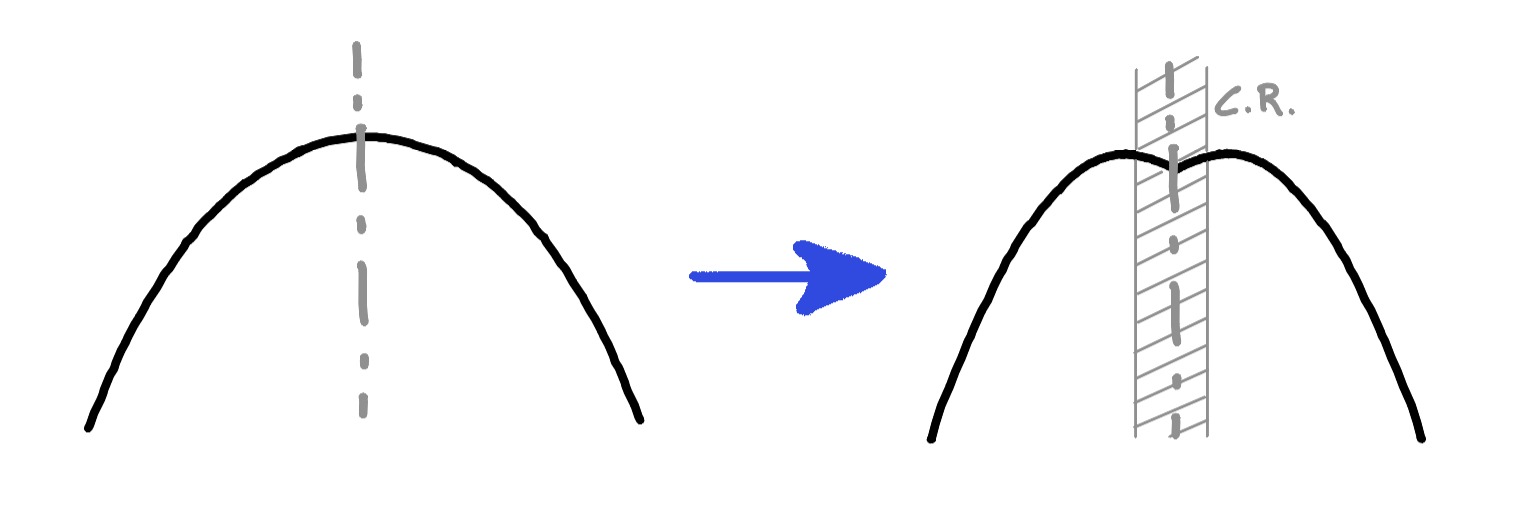
\includegraphics[width=0.75\linewidth]{CR_3.png}
    \caption{Flux before and after control rod insertion}
    \label{fig:flux_depression_cr_insertion}
\end{figure}

\textbf{Shadowing effect}: The position of one control rod can impact the effectiveness of another.

\subsection{Design}
The \textbf{material} selection is critical, requiring a substance with high absorption capabilities. For example, $B^{10}$ primarily undergoes (n,$\alpha$) reactions, while Gadolinium is more likely to produce (n,$\gamma$) reactions, which raises radiological safety concerns. \\
Following material selection, the \textbf{rod geometry} is typically constrained by overall design parameters. \\
Finally, the required \textbf{number of rods}, or equivalently the $pcm$, is determined by the need to compensate for excess reactivity at the start of the fuel cycle and provide an adequate shutdown margin. This depends on the core design and technology. 
For istance the difference between the excess reactivity over time in a conventional burner reactor agaist a breeeder reactor (shown in fig. \ref{fig:excess_reactivity_burner_vs_breeder}) shows the difference is needed reactivity compensation.

\begin{figure}[h]
    \centering
    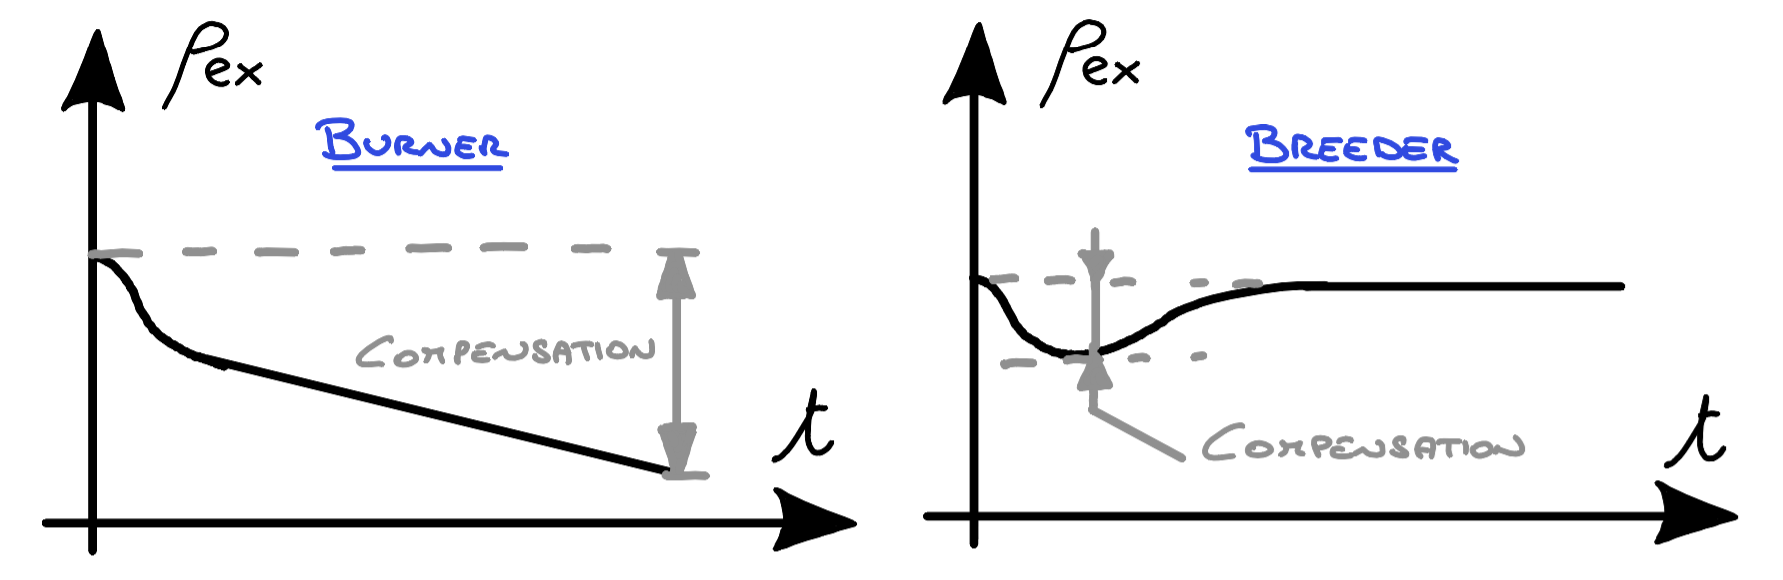
\includegraphics[width=0.75\linewidth]{CR_1.png}
    \caption{Reactivity worth needed for fuel consumption compensation is generally lower in breeder reactors compared to burner reactors.}
    \label{fig:excess_reactivity_burner_vs_breeder}
\end{figure}

\subsection{Calibration}
Calibration is necessary because the reactivity introduced by a control rod is not directly proportional to its insertion depth; instead, effectiveness varies with insertion depth, as illustrated in the following graphs:

\begin{figure}[h]
    \centering
    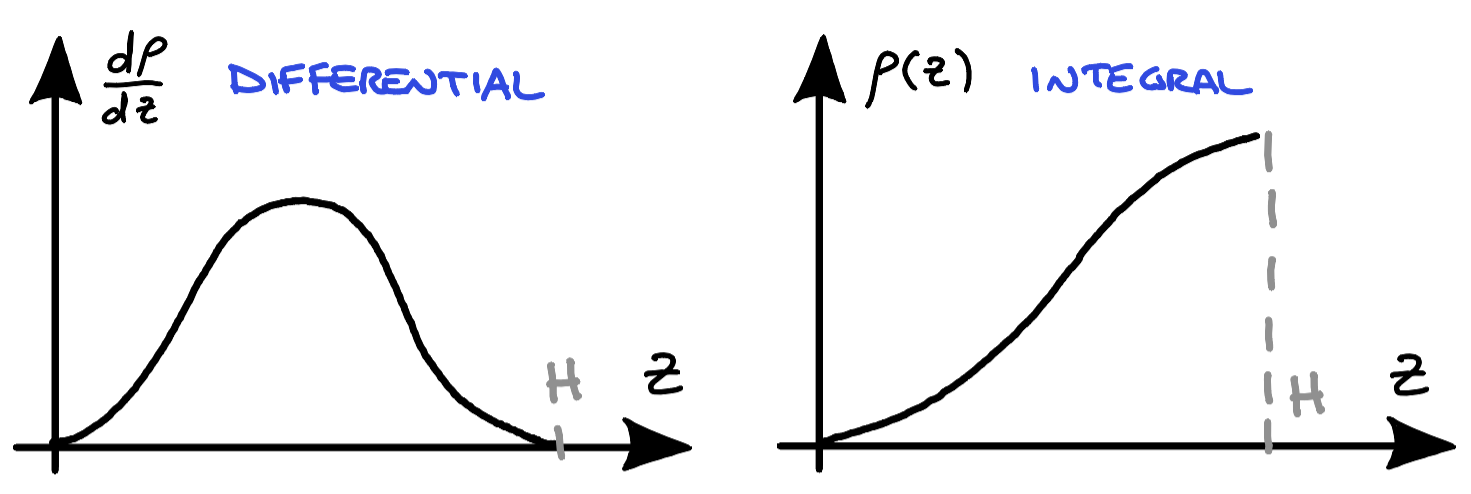
\includegraphics[width=0.75\linewidth]{CR_2.png}
    \caption{Differential and Integral reactivity curves}
\end{figure}


\subsection{Formulas}
The total reactivity worth ($\Delta \rho _{TOT}$) is given by:
\begin{equation}
    \Delta \rho _{TOT} = \Delta \rho _{SM} + \Delta \rho _{EX}
\end{equation}
where $\Delta \rho _{SM}$ is the shutdown margin and $\Delta \rho _{EX}$ is the reactivity excess.

Shutdown Margin:
\begin{equation}
    \Delta \rho _{SM} = \rho_i (\text{Criticality}) - \rho_i (\text{Fully IN}) 
\end{equation}
Reactivity excess:
\begin{equation}
    \Delta \rho _{EX} = \rho_i (\text{Fully OUT}) - \rho_i (\text{Criticality})
\end{equation}

\section{Critical Calibration Method}

\subsection{Theory}
The calibration of control rods in a reactor is crucial for understanding their reactivity worth. This can be accomplished using the in-hour and point kinetics equations to relate the time required to increase power by a factor to the reactivity.

\paragraph{Reactivity and Reactor Period}
The relationship between reactivity ($\rho$) and the reactor period ($T$) is fundamental in control rod calibration. The point kinetics equations describe this relationship:
\begin{equation}
    \frac{dP}{dt} = \frac{\rho - \beta}{\Lambda}P + \sum_{i=1}^6 \lambda_i C_i
\end{equation}
\begin{equation}
    \frac{dC_i}{dt} = \frac{\beta_i}{\Lambda}P - \lambda_i C_i
\end{equation}
where:
\begin{itemize}
    \item $P$ is the reactor power,
    \item $\rho$ is the reactivity,
    \item $\beta$ is the delayed neutron fraction,
    \item $\Lambda$ is the prompt neutron lifetime,
    \item $\beta_i$ and $\lambda_i$ are the delayed neutron fractions and decay constants for each of the six precursor groups,
    \item $C_i$ is the concentration of the $i$-th delayed neutron precursor group.
\end{itemize}

We can measure the reactor period $T$ by inserting a control rod and observing the time required for the reactor power to increase by a factor $e$. \\
In practice we will use a factor $1.5$ and compute the period as $T = \frac{\Delta t}{ln(1.5)}$. \\
We can then take advantage of the in-hour equation to correlate the reactivity to the reactor period:
\begin{equation}
    \rho = \frac{\Lambda}{\mathbf{T}} + \sum_{i=1}^6 \frac{\beta_i \lambda_i}{1 + \lambda_i \mathbf{T}}
\end{equation}
We are going to use a 6 group apprach, the values of $\beta_i$ and $\lambda_i$ are known from montecarlo simulations and therefore come with their own uncertanty.

\subsection{Pros and Cons of the Critical Method} 
    \textbf{Advantages}:
    \begin{itemize}
        \item Absolute method: results are independent of other factors, including the position of other control rods
        \item High accuracy of results 
    \end{itemize}
    \textbf{Disadvantages}: 
    \begin{itemize}
        \item Time-intensive, as calibration is required for each control rod
        \item Reactor remains in supercritical condition during measurements
    \end{itemize}

\subsection{Experimental Procedure}
Starting with a reactor in cold  and clean conditions to avoid effects due to external poisons or thermal feedback.
\begin{enumerate}
    \item Bring the reactor to a critical state.
    \item Raise the REG rod by some steps
    \item Measure the time required for the power to increase $3W \rightarrow 4.5W$.
    \item Measure the time required for the power to increase $6W \rightarrow 9W$.
    \item Adjust the shim rod to get back to criticality.
    \item Repeat until the REG rod is fully withdrawn.
\end{enumerate}
It is worth noting that the first measurment $3W \rightarrow 4.5W$ will take into also precursors, by the time 
of the second measurment most of them will be decayed so the measurment should be more rapresentative of the reactiviy. \\
\section{Subcritical Control Rod Calibration}

\subsection{Introduction}
The subcritical method provides an alternative approach to control rod calibration, particularly useful for cases where safety is a concern. 
This method allows for calibration while keeping the reactor in a subcritical state by using an external neutron source.

\subsection{Theory - TBC}
\paragraph{Subcritical Multiplication and Reactor Period}
In subcritical conditions, the neutron population depends on both the external source and the reactor’s multiplication factor $K_{eff}$. This dependency is described by the subcritical multiplication factor $M$:
\begin{equation}
    M = \frac{1}{1 - K_{eff}}
\end{equation}
With an external source, the neutron population evolves over generations until it reaches a steady state. 
This evolution can be described by a geometric series with $K_{eff}$ as the ratio, where the number of generations required to reach steady state is:
\begin{equation}
    N_{\text{steady}} \approx \frac{4}{\ln K}
\end{equation}
Which means that the evolution is slower the closer we get to the steady state condition.

\paragraph{Point Kinetics Equations}
To understand the reactor's response over time, we use the point kinetics equations adapted for the subcritical state:
\begin{equation}
    \frac{dn}{dt} = K_{eff} \left( \frac{K_{eff} - 1}{K_{eff}} + \rho - \beta \right) \frac{n}{\Lambda} + \sum \lambda_i C_i + q
\end{equation}
\begin{equation}
    \frac{dC_i}{dt} = K_{eff} \frac{\beta_i}{\Lambda} n - \lambda_i C_i
\end{equation}
where $\rho = \frac{\Lambda}{K}$ and $q$ is the source term. The reactor period $T$ is then given by:
\begin{equation}
    T = \frac{1}{\lambda_1}
\end{equation}

\subsection{Experimental Procedure}
The following steps outline the subcritical calibration procedure:
\begin{enumerate}
    \item Bring the reactor in subcritical condition with all rods inserted.
    \item Measure the neutron rate $\dot{R}$, we used a fission chamber, in pulse mode.
    \item Insert the source and measure $\dot{R}$ again, we used $Ra\text{-}Be$,.
    \item Extract the control rods of which we know its reactivity worth and measure $\dot{R}$ once it reached steady state.
    \item Compute the subcritical multiplication factor of the CR from known reactivity worth: $\Delta \rho = \rho_{out} - 0 = \frac{K - 1}{K} \rightarrow M = \frac{1}{1 - K}$.
    \item Compute the calibration parameter $\alpha \Phi_s$ from this measurment: $\frac{\dot{R}}{M} = \alpha \Phi_s$.
    \item Reinsert the control rod.
    \item Extract another control rod and measure $\dot{R}$.
    \item Compare measured $\dot{R}$ to the calibration parameter: $M = \alpha \Phi_s \dot{R}$
    \item Repeat the last two steps for all control rods.
\end{enumerate}
For better statistics take multiple measurements for each control rod (or long measurements).

\begin{tcolorbox}[boxstyle2]
    \textbf{Note on statistics}:
    In poisson distributed data like radiation counts taking 20 short measurments each of time $t$ will give the same statistical error
    as taking 1 longer measurement of time $T = 20t$.
\end{tcolorbox}


\subsection{Pros and Cons of the Subcritical Method}
    \textbf{Advantages}:
    \begin{itemize}
        \item Safe and keeps the reactor subcritical.
        \item Allows calibration of the shim, unlike other methods.
    \end{itemize}
    \textbf{Disadvantages}:
    \begin{itemize}
        \item Relys on the knowledge of one control rod's reactivity worth.
        \item Lower accuracy due to reliance on source and instrumentation.
        \item Only measures the total worth of the control rod, unable to get the full integral curve with reasonable measuring time (if we do a small step the variation in count rate change can easly hide in the noise and error).
        \item Frequent recalibration required due to burnup of fission chamber.
    \end{itemize}
\chapter{Reactivity Coefficients}
\section{Definition}

The reactivity coefficient, denoted as $\alpha$, is defined as:
\begin{equation}
    \alpha = \frac{\partial \rho}{\partial x}
\end{equation}
where $x$ represents a certain quantity that affects the reactivity, $\rho$.

\section{Reactivity Coefficients for Different Components}

For our case, we consider the following reactivity coefficients.

\begin{itemize}
    \item $\alpha_f$ = Fuel reactivity coefficient
    \item $\alpha_m$ = Moderator reactivity coefficient
    \item $\alpha_c$ = Coolant reactivity coefficient
    \item $\alpha_e$ = Reactivity due to thermal expansion of the fuel
\end{itemize}

In the TRIGA reactor, $\alpha_e$ can often be neglected because, as in other thermal systems, the thermal expansion is smaller compared to the migration length of neutrons.

\begin{tcolorbox}[boxstyle2]
\textbf{Note for fast reactors:} The higher migration length in fast reactors makes the reactivity effect of thermal expansion more relevant.
\end{tcolorbox}

\section{Doppler Effect}

The fuel reactivity coefficient, $\alpha_f$, is primarily due to the Doppler effect. The Doppler effect causes a broadening of the resonance peaks in the absorption cross-section of the fuel.

\begin{equation}
    \sigma(\text{fuel, E}) = \text{Doppler Effect}
\end{equation}

\begin{figure}[h]
    \centering
        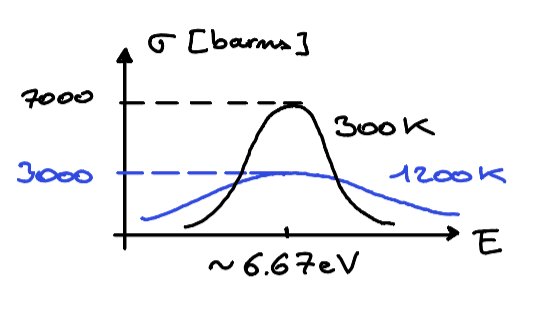
\includegraphics[width=0.75\linewidth]{doppler.png}
    \caption{The Doppler effect shows the broadening of resonance peaks.}
\end{figure}

\section{Functions of Reactivity Coefficients}

Specifically for the TRIGA reactor:
\begin{itemize}
    \item $\alpha < 0$ indicates a \textbf{negative reactivity coefficient}, which is essential for safety.
    \item $\alpha \ll 0$ allows for stable operation in \textit{pulse mode}.
\end{itemize}

\section{Design Considerations}

When designing a system with fuel and moderator, consider the following:
\begin{itemize}
    \item Increase in temperature ($T \uparrow$) leads to reduced moderation capability, affecting the neutron flux.
    \item The effect on the absorption cross-section ($\Sigma_a \downarrow$) also reduces the reactivity.
\end{itemize}

\section{Physical Background}

The physical background involves the following dynamics:
\begin{equation}
    \frac{dn}{dt} = P - A - L + S
\end{equation}
where:
\begin{itemize}
    \item $P$ denotes production, which depends on $\Sigma_f \phi$
    \item $A$ denotes absorption, proportional to $\Sigma_a \phi$
    \item $L$ denotes leakage, related to $\nabla D \phi$
    \item $S$ denotes scattering, related to $\Sigma_s \phi$
\end{itemize}

The reactivity $\rho$ can be approximated by:
\begin{equation}
    \rho \propto \frac{P - A - L}{P}
\end{equation}

\subsection{Dependence on Parameters}

The parameters affecting reactivity are:
\begin{itemize}
    \item Temperature (affects cross-section and density)
    \item Geometry (affects distribution)
    \item Fuel condition (corrosion, burnup, etc.)
\end{itemize}

\subsection{Side Note on Fast Reactors}

In fast reactors, the coefficients $\alpha_f$ and $\alpha_c$ can be greater than zero depending on the fuel composition, as is the case with molten salt reactors where fuel is mixed with the coolant.

\section{Overview of the Effects of Reactivity Coefficients}

The following plot gives an overview of how reactivity feedbacks affect power in the reactor.
\begin{figure}[H]
    \centering
        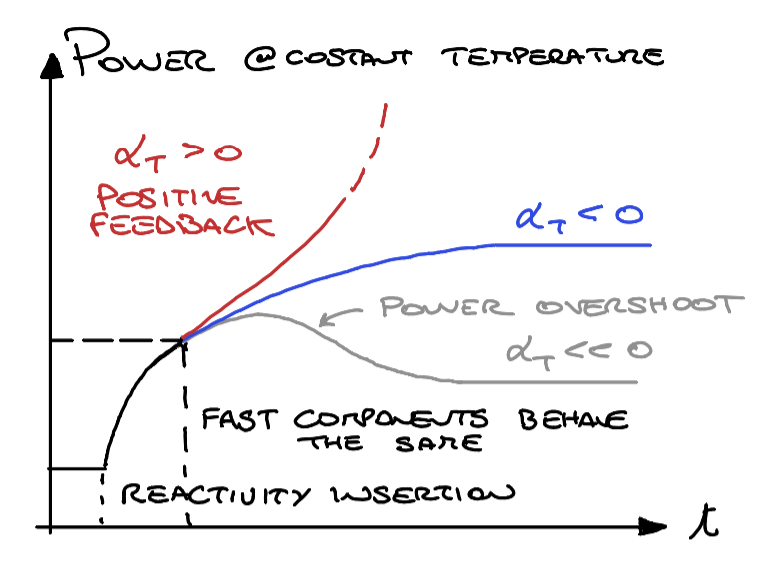
\includegraphics[width=0.6\linewidth]{power_effect.png}
    \caption{Overview of the effects of $\alpha$ on reactor power.}
\end{figure}

\section{TRIGA Fuel}

TRIGA fuel consists of Uranium-Zirconium Hydride (U-Zr-H), the solid moderator comprises hydrogen, with zirconium acting as the stabilizing element.

\subsection{Experimental Findings}

\paragraph{First Experiment: Mono-Energy Neutron Source}: Determination of the effective energy for moderation. \\
\paragraph{Second Experiment: Acoustical Resonance Study}: Influence of temperature on resonance peaks. \\
\paragraph{Third Experiment: Cross-Section Evaluation}: Measuring total removal cross-section.

\section{Explanation of the Results}

The findings from these experiments suggest that:
\begin{enumerate}
    \item Hydrogen in a lattice has no free recoil.
    \item The interference effect is characterized by a wavelength related to specific energy levels.
    \item Possibility of up-scattering due to vibration modes.
\end{enumerate}

\section{Thermalization through Bounded Nuclei}

The thermalization process occurs via two primary pathways:
\begin{enumerate}
    \item \textbf{Translation Modes}:
        \begin{itemize}
            \item Elastic interaction involving the entire crystal structure.
            \item Reduced logarithmic energy decrease with increased temperature.
        \end{itemize}
    \item \textbf{Vibration Modes}:
        \begin{itemize}
            \item Excitation of vibration states that influence up-scattering.
        \end{itemize}
    \item \textbf{Coherent and Incoherent Scattering}
\end{enumerate}

The total scattering cross-section, $\sigma_{\text{scattering}}$, consists of both coherent and incoherent components:
\begin{equation}
    \sigma_{\text{scattering}} = \sigma_{\text{coherent}} + \sigma_{\text{incoherent}}
\end{equation}
In the TRIGA reactor
\section{Elastic vs Inelastic Scattering}

Elastic scattering involves no change in the internal quantum states of the scatterer. In contrast, inelastic scattering involves changes in these states.

\begin{itemize}
    \item \textbf{Elastic}: No excitation states, such as with free hydrogen.
    \item \textbf{Inelastic}: Involves excitation related to vibrations and rotations within the molecule.
\end{itemize}

\section{Thermalization through Bounded Nuclei}

Thermalization of neutrons through bounded nuclei can occur via two primary mechanisms:
\begin{enumerate}
    \item \textbf{Translation Modes}:
        \begin{itemize}
            \item Elastic interactions that involve the entire crystal lattice.
            \item Changes in temperature lead to variations in logarithmic energy decrease.
        \end{itemize}
    \item \textbf{Vibration Modes}:
        \begin{itemize}
            \item Specific energy excitations related to vibrational modes.
            \item Absorption of vibrational energy quanta can lead to up-scattering.
        \end{itemize}
\end{enumerate}

\section{Coherent and Incoherent Scattering}

Coherent scattering occurs when scattering events result in interference effects due to the crystal structure, manifesting as Bragg peaks. Incoherent scattering, in contrast, lacks such regular interference patterns.

\begin{equation}
    \sigma_{\text{scattering}} = \sigma_{\text{coherent}} + \sigma_{\text{incoherent}}
\end{equation}

\begin{figure}[h]
    \centering
    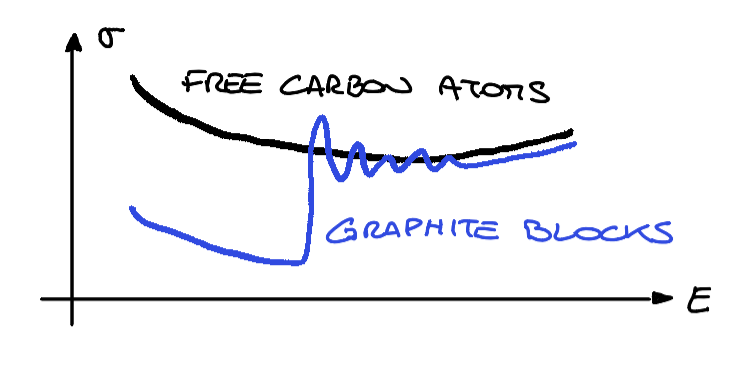
\includegraphics[width=0.75\linewidth]{coherent_vs_inchoerent.png}
    \caption{Coherent and incoherent scattering on Carbon atoms, when they form a crystalline structure in the graphite the scattering is inchoerent.}
\end{figure}

\section{Summary of Findings on TRIGA Fuel}

The experimental findings on TRIGA fuel reveal key insights into moderation and reactivity:

\begin{itemize}
    \item TRIGA fuel demonstrates effective moderation properties above a certain energy threshold.
    \item The presence of zirconium hydride contributes significantly to the observed moderation effects.
    \item Doppler effects and up-scattering play important roles in spectral hardening.
\end{itemize}

\section{Recap of Results}

To summarize, the moderation capabilities of hydrogen in zirconium hydride are influenced by several factors, including lattice structure and vibrational modes. Based on experiments and Monte Carlo simulations:

\begin{itemize}
    \item The Bragg peak is negligible in the energy range of interest.
    \item The primary mechanism involves vibrational modes related to the hydrogen lattice.
    \item Spectral hardening is observed with increasing temperature.
\end{itemize}

\begin{tcolorbox}[boxstyle2]
The findings suggest that Zr-H-based fuels exhibit complex moderation behavior, particularly at higher temperatures where vibrational modes play a significant role.
\end{tcolorbox}

\section{Additional Notes}

\subsection{Composition of fuel reactiviy coefficent in the TRIGA reactor}

A breakdown of the contributions to $\alpha_f$ in the TRIGA reactor is presented in the table below.

\begin{table}[h]
    \centering
    \begin{tabular}{|l|c|c|}
        \hline
        Contribution & Aluminum Cladding & Stainless Steel Cladding \\
        \hline
        Doppler Effect & 2.6 & 2.1 \\
        Spectral Hardening & 5.7 & 7.8 \\
        Cell Flux Effect & 3.5 & 5.7 \\
        Leakage Effect & 2.2 & 2.1 \\
        \hline
        Total $\alpha_f$ (pcm/°C) & 8.3 & 9.9 \\
        \hline
    \end{tabular}
    \caption{Breakdown of $\alpha_f$ contributions in TRIGA for different cladding materials.}
\end{table}

\subsection{TRIGA Fuel Characteristics}
TRIGA fuel (Zr-H) can moderate up to 0.13 eV and can induce upscattering, as indicated by experimental evidence, which justifies the use of H\textsubscript{2}O as a moderator.

\begin{itemize}
    \item Hydrogen is bounded to Zr, and for thermal energy, the bound cannot be neglected.
    \item Hydrogen in Zr-H moderates mainly through inelastic scattering.
    \item \textbf{Model:} Using the Einstein quantum harmonic oscillator, we can explain the experimental evidence.
\end{itemize}

In TRIGA fuel, the temperature coefficient $\alpha_T$ is approximately $-7$ to $-9$ pcm/°C.

\section{Experimental Brief}
\begin{itemize}
    \item \textbf{Step 1:} Shift out control rods $\rightarrow$ $\rho \uparrow$ $\rightarrow$ Power $\uparrow$
    \item \textbf{Step 2:} Overshoot of power is observed.
    \item \textbf{Step 3:} Compute the energy release up to the peak.
    \item \textbf{Step 4:} Estimate the temperature $T$.
    \item \textbf{Step 5:} Compute the temperature coefficient $\alpha_T$.
\end{itemize}

Note: The coolant temperature coefficient, $\alpha_{T_{\text{coolant}}}$, is slightly positive.

\section{Void Coefficient}

\subsection{Definition and Function}
The void coefficient, $\alpha_v$, is defined as:
\begin{equation}
    \alpha_v = \frac{\partial \rho}{\partial \mathcal{E}}
\end{equation}
where $\mathcal{E}$ represents the void fraction. The void coefficient plays an important role in safety, helping assess the response in situations like boiling, experiments, irradiation, and Loss of Coolant Accidents (LOCA).

\subsection{Design Considerations and Physical Background}
\begin{itemize}
    \item Changes in moderation due to void formation lead to spectral hardening, causing a decrease in the resonance escape probability $p$.
    \item Absorption decreases, increasing the thermal utilization factor $f$.
    \item Leakage increases, reducing the probability of non-leakage $P_{NL}$.
\end{itemize}

\begin{figure}[H]
    \centering
    
\includegraphics[width=0.75\linewidth]{placeholder.png}
    \caption{Effect of moderation ratio on $k_{\text{eff}}$.}
\end{figure}

\section{Impact on the Six-Factor Formula}

\begin{itemize}
    \item $p$: Resonance escape probability
    \begin{equation}
        \alpha_{p,i} = \ln \left( \frac{1}{p} \right) \left( \frac{1}{N_H V_H} \frac{\partial N_H V_H}{\partial V} \right) = \frac{\partial p}{\partial V}
    \end{equation}
    
    \item $f$: Thermal utilization factor
    \begin{equation}
        \alpha_{f,i} = (1 - f) \left( - \frac{1}{N_H V_H} \frac{\partial N_H V_H}{\partial V} \right)
    \end{equation}
\end{itemize}

These coefficients are strongly dependent on absorption and moderation capacity. For example:
\begin{itemize}
    \item \textbf{Void in Fuel} $\rightarrow \rho \downarrow$
    \item \textbf{Void in Water} $\rightarrow \rho \uparrow$
\end{itemize}

\section{Experiment Outline}
\begin{enumerate}
    \item Start at zero power, aiming to create a void.
    \item Ensure zero power, clean, and critical conditions.
    \item Register control rod positions.
    \item Insert a sample filled with water:
    \begin{itemize}
        \item If $\alpha_v < 0$, $\rho \uparrow$
    \end{itemize}
    \item Return to criticality by adjusting the control rods.
    \item Find control rod calibration curves to determine $\Delta \rho$.
\end{enumerate}

\textbf{Samples:} Placed in one of the channels.

\subsection{Examples of Void Experiments}
\begin{itemize}
    \item \textbf{In Ljubljana:} Bubbles were injected into the core. Monte Carlo simulations confirmed that $\alpha_v < 0$.
    \item \textbf{In Vienna:} Fuel elements with 70\% enrichment were used, making $\alpha_v > 0$ due to high enrichment and the limited need for moderation.
\end{itemize}

\section{Effects on Neutronics}

The reactivity $k$ can be expressed as:
\begin{equation}
    k = \eta f \epsilon P_{NL} P_{NL}
\end{equation}

The differential of $k$ with respect to a parameter $x_i$ can be expanded:
\begin{equation}
    \alpha_i = \frac{\partial \rho}{\partial x_i} = \frac{1}{k} \frac{\partial k}{\partial x_i} = \frac{1}{\eta} \frac{\partial \eta}{\partial x_i} + \frac{1}{f} \frac{\partial f}{\partial x_i} + \frac{1}{\epsilon} \frac{\partial \epsilon}{\partial x_i} + \dots
\end{equation}

\begin{itemize}
    \item \textbf{Doppler Effect:} Variations in resonance weight due to self-shielding.
    \item \textbf{Spatial Self-Shielding:} Outer rings of the fuel pin shield the center, reducing the flux at the core.
\end{itemize}

\section{Spectral Hardening}

Spectral hardening occurs due to the harmonic oscillator behavior of Zr-H:
\begin{equation}
    \alpha_{f,i} \approx \frac{1}{\Sigma_a^f} \frac{\partial \Sigma_a^f}{\partial x_i} - \frac{1}{\Sigma_a^m} \frac{\partial \Sigma_a^m}{\partial x_i} - \frac{1}{\phi} \frac{\partial \phi}{\partial x_i}
\end{equation}

In fuel, spectral hardening increases the mean free path, affecting capture and escape probabilities.

\subsection{Disadvantage Factor}
\begin{equation}
    \zeta = \frac{\phi_{\text{moderator}}}{\phi_{\text{fuel}}}
\end{equation}

Since spectral hardening is stronger in the fuel, the ratio of escaping flux from the fuel is higher.

\section{Experimental Procedure}

This procedure yields a reactivity temperature coefficient rather than a prompt fuel coefficient.

\begin{itemize}
    \item Measure $\Delta T$ due to $\Delta \rho$ and compute the ratio.
    \item No direct way to measure $T_f$ (limited thermocouples, coolant contribution).
\end{itemize}

\subsection{Simple Approach}
\begin{enumerate}
    \item Set reactor at desired power.
    \item Record control rod position and extract positive reactivity.
    \item Record power variation.
    \item Calculate energy released until peak.
    \item Calculate average temperature difference.
    \begin{equation}
        \Delta T_f = \frac{E}{G_f(N_f)}
    \end{equation}
    \item Calculate the $\beta$ temperature coefficient.
\end{enumerate}

\section{Coolant Effects}

\subsection{Components}
Two contributions:
\begin{itemize}
    \item Water density decrease, leading to $\rho \downarrow$
    \item Different rod capacity of H in water, leading to $\rho \uparrow$
\end{itemize}

Overall, $\alpha_{T_{\text{coolant}}} < 0$, although some contributions can be positive.

\subsection{Isothermal Coefficient}
\begin{equation}
    \alpha_{\text{iso}} = \alpha_{T_f} + \alpha_{T_c}
\end{equation}
Observed in Ljubljana by changing pool conditions while maintaining core conditions.

\begin{equation}
    \alpha_{\text{iso}} = -3 + 6.5 = +3.5 \text{ pcm/°C}
\end{equation}

\textbf{Experimental Note:} Despite positive contributions, $\alpha_{T_c} < 0$ overall.

\chapter{Pulse Mode}
\chapter{Pulse Mode}

\section{Pulse Mode Operation}
In pulse mode operation, the reactor is driven into a short, high-intensity power pulse. This mode is characterized by:
\begin{itemize}
    \item Short duration
    \item High intensity
\end{itemize}
The observed parameters in pulse mode include:
\begin{enumerate}
    \item Power (Intensity)
    \item Time to reach peak power (to compare pulse duration)
    \item Full Width at Half Maximum (FWHM) of the pulse
\end{enumerate}

\begin{figure}[H]
    \centering
    
\includegraphics[width=\textwidth]{placeholder.png}
    \caption{Illustration of pulse mode operation with parameters like peak power and FWHM.}
    \label{fig:pulse_mode}
\end{figure}

\section{Functions of Pulse Mode}
Pulse mode can be used for various purposes, including:
\begin{itemize}
    \item Activation analysis, including detector or semiconductor analysis
    \item Safety tests, such as reactivity insertion accidents
    \item Estimation of parameters related to reactor kinetics
\end{itemize}

\section{Physical Background}
In the pulse mode, the following sequence occurs:
\begin{align*}
    \rho \uparrow \to P \uparrow \to E(T) \to T \uparrow \to \alpha_T \to \rho \downarrow \to \text{Feedback stabilizes the system.}
\end{align*}
To translate energy into temperature, we need to know the heat capacity, $C_p$. The other important parameter is the temperature reactivity coefficient, $\alpha_f$.

\section{Experimental Evidence of Ljubljana Pulses}
Videos of different reactivity insertions in the Ljubljana TRIGA reactor show that:
\begin{itemize}
    \item Higher intensity in Cherenkov radiation correlates with larger $\Delta \rho$.
    \item Shorter pulses are achieved with larger $\Delta \rho$.
    \item The reactor is always scrammed after each pulse for safety, even if it is self-limited.
\end{itemize}
The Nordheim-Fuchs model is employed to understand the self-limited excursions during these pulses. The model incorporates several key assumptions:
\begin{enumerate}
    \item Transients are modeled using point kinetics.
    \item Delayed neutrons are neglected due to the short timescale.
    \item The reactivity insertion, $\Delta \rho$, is treated as a step function.
    \item Adiabatic heat transfer is assumed for the energy balance, focusing on the heat transfer to the coolant over a characteristic timescale.
\end{enumerate}
The adiabatic assumption is valid only from a global perspective, as local variations in fission rates across individual fuel elements can lead to higher localized heat transfer coefficients (HTCs). This highlights the importance of understanding local phenomena in addition to the overall system behavior.

\section{Nordheim-Fuchs Model}
The Nordheim-Fuchs model is used to understand self-limited excursions over a short timespan. It relies on several assumptions:
\begin{enumerate}
    \item Transient modeled with point kinetics
    \item Delayed neutrons are neglected
    \item $\Delta \rho$ is considered a step function
    \item Adiabatic model for energy balance
\end{enumerate}

\begin{figure}[H]
    \centering
    
\includegraphics[width=\textwidth]{placeholder.png}
    \caption{Power pulse prediction by Nordheim-Fuchs model showing peak power and pulse duration.}
    \label{fig:nordheim_fuchs}
\end{figure}

\subsection{Derivation of the Nordheim-Fuchs Model}
The derivation of the Nordheim-Fuchs model begins with several simplifying assumptions:
\begin{enumerate}
    \item Point kinetics approximation is used, ignoring spatial effects.
    \item Delayed neutrons are neglected ($C_i = 0$) due to the short timescale of the pulse.
    \item No external neutron source is present ($S = 0$).
    \item Reactivity insertion, $\rho(t)$, is treated as a step function: $\rho(t) = \rho_0 H(t)$.
    \item Heat transfer is modeled adiabatically, assuming no heat loss during the transient.
\end{enumerate}
The rate of change of reactivity is given by:
\begin{align*}
    \frac{dP}{dt} = \frac{\rho - \beta}{\Lambda}P,
\end{align*}
where $P$ is the power, $\beta$ is the delayed neutron fraction, and $\Lambda$ is the prompt neutron lifetime. 

For the temperature feedback:
\begin{align*}
    \rho = \rho_0 - \alpha(T_f - T_{f,0}),
\end{align*}
where $\alpha$ is the temperature reactivity coefficient and $T_f$ is the fuel temperature. Using the adiabatic heat transfer model:
\begin{align*}
    \frac{dT_f}{dt} = \frac{P}{m_f c_{p,f}},
\end{align*}
where $m_f$ is the fuel mass and $c_{p,f}$ is the specific heat capacity. Combining these equations leads to a coupled differential system that can be solved for $P(t)$ and $T_f(t)$.

After integration, the peak power and the Full Width at Half Maximum (FWHM) of the pulse can be derived:
\begin{align*}
    P_{\text{max}} &= \frac{m_f c_{p,f}}{\alpha}\left(\rho_0^2 - \beta^2\right), \\
    \text{FWHM} &= 3.52\sqrt{\frac{\Lambda}{\alpha m_f c_{p,f}}}.
\end{align*}
These expressions highlight the dependence of pulse characteristics on reactor parameters such as $\rho_0$, $\alpha$, and $m_f$.

\section{Power Pulse Parameters}
The key parameters of a power pulse are:
\begin{itemize}
    \item $\Delta \rho$: Known insertion value
    \item $T_f$: Fuel temperature from instrumentation
    \item $E_{\text{released}}$: Power integral for total energy release
\end{itemize}

\section{Why TRIGA Can Operate in Pulse Mode}
The TRIGA reactor can safely operate in pulse mode due to:
\begin{itemize}
    \item Large prompt and negative temperature coefficient, $\alpha_f = -8$ to $-10$~pcm/K
    \item High heat capacity of the fuel-moderator combination
\end{itemize}
Note: In the Ljubljana TRIGA reactor, fewer control rods and elements with higher uranium content allow a unique pulse operation configuration.

\section{Physical Phenomenon of the Pulse}
The physical phenomenon during a pulse involves:
\begin{enumerate}
    \item Large $\rho$ insertion ($> 2\$$)
    \item Prompt supercriticality reached
    \item Fuel temperature increases, causing $\rho \downarrow$ until stability
\end{enumerate}

\begin{figure}[h]
    \centering
    
\includegraphics[width=\textwidth]{placeholder.png}
    \caption{Graph showing power pulse parameters and energy release.}
    \label{fig:power_pulse}
\end{figure}

\section{Examples and Limitations}
Examples of the results from the Nordheim-Fuchs model indicate:
\begin{itemize}
    \item Increasing $\rho_0$ leads to higher peak power, reduced FWHM, increased energy in fuel, and larger $\Delta T_f$.
\end{itemize}

Limitations of this model include:
\begin{itemize}
    \item For slow pulses, delayed neutrons are no longer negligible, and their impact must be accounted for.
    \item The heat capacity, $C_p$, actually depends on the temperature, introducing non-linearities that the model does not capture.
    \item The model does not account for ramped reactivity insertions, assuming a step-like reactivity input instead.
    \item The point kinetics assumption ignores spatial effects, which may become significant in certain configurations.
    \item Experimental validation shows deviations in scenarios where local thermal feedback or hydrodynamic effects dominate.
\end{itemize}

\section{Experimental Procedure}
The following steps outline the experimental procedure for conducting pulse mode experiments:
\begin{enumerate}
    \item Establish critical conditions with the transient rod inserted, then fully withdraw the transient rod to initiate the pulse.
    \item Maintain the reactor at low power (approximately 1000 W) to avoid shadowing effects during the step insertion.
    \item Fire the pulse by extracting the transient rod using the fast pneumatic system.
    \item Scram the reactor approximately 15 seconds after the pulse to ensure safety.
    \item Wait for the reactor to cool down before proceeding with further operations.
\end{enumerate}

%%%%%%%%%%%%%%%%%%%%%%%%%%%%%%%%%%%%%%%%%%%%%%%%%%%%%%%%%%%%

%%%%%%%%%%%%%%%%%%%%%%%%%%%%%%%%%%%%%%%%%%%%%%%%%%%%%%%%%%%%
%
%%%%%%%%%%%%%%%%%%%%%%%%%%%%%%%%%%%%%%%%%%%%%%%%%%%%%%%%%%%%

\end{document}
